\section{Introduction}
To first get an understanding of why this project was done, it is important for the reader to learn, not only the background of the fields studied, but also about the prospects of the technologies involved.
 At \hyperref[subsecBackground]{3.1} we go through the current and the potential use of these technologies; also what prospects the consumers and the industry have. Later on, at  \hyperref[subsecPrevStud]{3.2} we go through some of the previous research that has been done in the fields that are studied in the report. This section is then rounded off at \hyperref[subsecGoal]{3.3} with us telling you what we hoped to achieve with this project and a brief run-down of how.
 
 The full repository for this project can be downloaded at \url{https://github.com/iSadist/master-thesis}

\subsection{Background}
\label{subsecBackground}
The idea of Augmented Reality is to render virtual object in the real world. This usually requires hardware in the form of a camera and display, a processing unit and software. Common AR devices today are the HoloLens \cite{microsoft}, Google's Glass \cite{googleGlasses} and a vast amount of mobile devices, such as Apple's iPhone X \cite{appleAR}. 

The general interest for AR has undeniably grown in recent years, with mobile games and applications such as Niantic's Pokémon Go \cite{pokemonGO} and IKEA's IKEA Place \cite{IKEAPlace} the AR industry has peaked a general interest and sources speculate it could be a \$90 million dollar industry by 2022 \cite{digi-capital}.
 But Augmented Reality has not only reached the casual users; the technology has also peaked an interest in several industries. One such project is Fieldbit's Fieldbit Hero \cite{fieldbit}, a platform enabling technicians to get instant AR annotations to their AR devices from an engineer, allowing the technician to get visual instructions while simultaneously  being able to work hands-free. 
 
However, as of now, most localization and identification of objects within AR are done using marker detection \cite{markerDetection}. An alternative to this would be to use \textit{Deep Neural Networks}, as they have been proven to be very useful for object detection in images. The hype around neural networks has been particularly strong since AlexNet scored high in the ImageNet LSVRC-2010 challenge and the ImageNet ILSVRC-2012 challenge \cite{NIPS2012_4824}. They accomplished these feats by making use of new methods, e.g. \textit{dropout}. Since then several different types of network models have been created. Now we have network models that can detect both where an object is in an image, and what the object is, in one go. One such network is \textit{YOLO}\cite{YOLO1}. By adopting such a network, the need for having to mark objects would drop significantly and it would open up for many more possible use cases for AR.
 
\subsection{Previous studies}
\label{subsecPrevStud}
D. Chatzopoulos et al.(2017) describes the basics of Mobile Augmented Reality, its advancements and it's flaws. They estimate that MAR is the most promising field of mobile applications and that it will have a massive impact on how we interact with the real world. However, they also go through some of the current hiccoughs with the technology, such as bandwith limitation and the computing power required. 
\cite{MARS}

S.Gould et al.(2009) writes about a hierarchical model for joint object detection and image segmentation, where they basically tried to segment all objects in an image and classifies every pixel. 
\cite{NIPS2009_3766}


Y LeCun and M.A. Ranzato goes in-depth on the history and progress of deep learning, from the first machine learning model, the Perceptron, to future challenges with deep learning. They write about the use cases for machine learning and how models generally work. They also classify different kinds of models into separate categories. Also written about is areas such as what makes a good feature and how convolutional neural networks are constructed.
\cite{deepLearningTutorial}


\subsection{The goal of this project}
\label{subsecGoal}
Our goal is to try to combine Augmented Reality with Object detection and Object recognition to find out if it is feasible and if there is an actual desirable use case for this technique. 

This will be limited to the use of ARKit 2 developed by \textit{Apple} for iOS devices. An augmented reality application for iPhone X incorporating the use of modern machine learning models for object detection and recognition will be developed in order to test our thesis. The application will be an assembly manual for furniture. Deep neural networks will be trained to recognize the different available parts and configurations of said parts.  The model should then predict which parts it is seeing in the camera feed, where they are and show how they should be assembled in an AR scene. 

Hence, we will not research what is possible with other hardware, although, we will mention them. We will also restrict the amount of furniture we train on, as well as the environments they will be built in. However, we hypothesize that if it works for one furniture and one set of environments, it should be possible to scale for larger sets.


\subsection{Jayway}
This project is conducted partly on Jayway's request and much of the work is done in their office in Malmö.
Jayway is a software studio with offices in Malmö, Halmstad, Stockholm, Copenhagen and Palo Alto. They aim to provide costumers with digital solutions  within fields such as mobile, web, backend, cloud as well as UX \& design. They also have a focus on AR \& VR, where they hope to give businesses a new perspective on the technologies.

%Quote?

The purpose of this project for Jayway is mainly to explore Object Recognition  and ARKit, and how they could be combined together to create value. The main question is to know, if possible, how easy it is to implement a solution.
Jayway is continuously looking to explore new technologies and Augmented Reality is a hot new trend emerging in the markets in the time of writing this report.
A second objective is for Jayway to take the finished implementation to one of their customers and
present an example of what they are able to do for their customers.

\newpage


\subsection{Summary of our plans}
In order to start a project of this magnitude, a good strategy had to be conceived. 

\subsubsection{Mock-up of the planned product}
To be able to design the layout and flow of the application, a mock-up of application was first created, illustrating the information and use flow throughout the usage. In this section the general concept will be described and why it was designed in this way. The mock up was created using a free online tool called MockFlow\cite{mockflow}. 

When the application is opened up, one is taken to a furniture selection screen, see figure \ref{fig:furniture-select}, which allows the user to select which furniture they want to assemble. A user can select the furniture by either scrolling through the list, using the search bar, or using the built in barcode scanner. It was important for a first time user to understand what the purpose of the application was when they first open up the app. Therefore, first time users are greeted with an informative pop-up notification explaining the general purpose.

\begin{figure}[hbtp]
\begin{center}
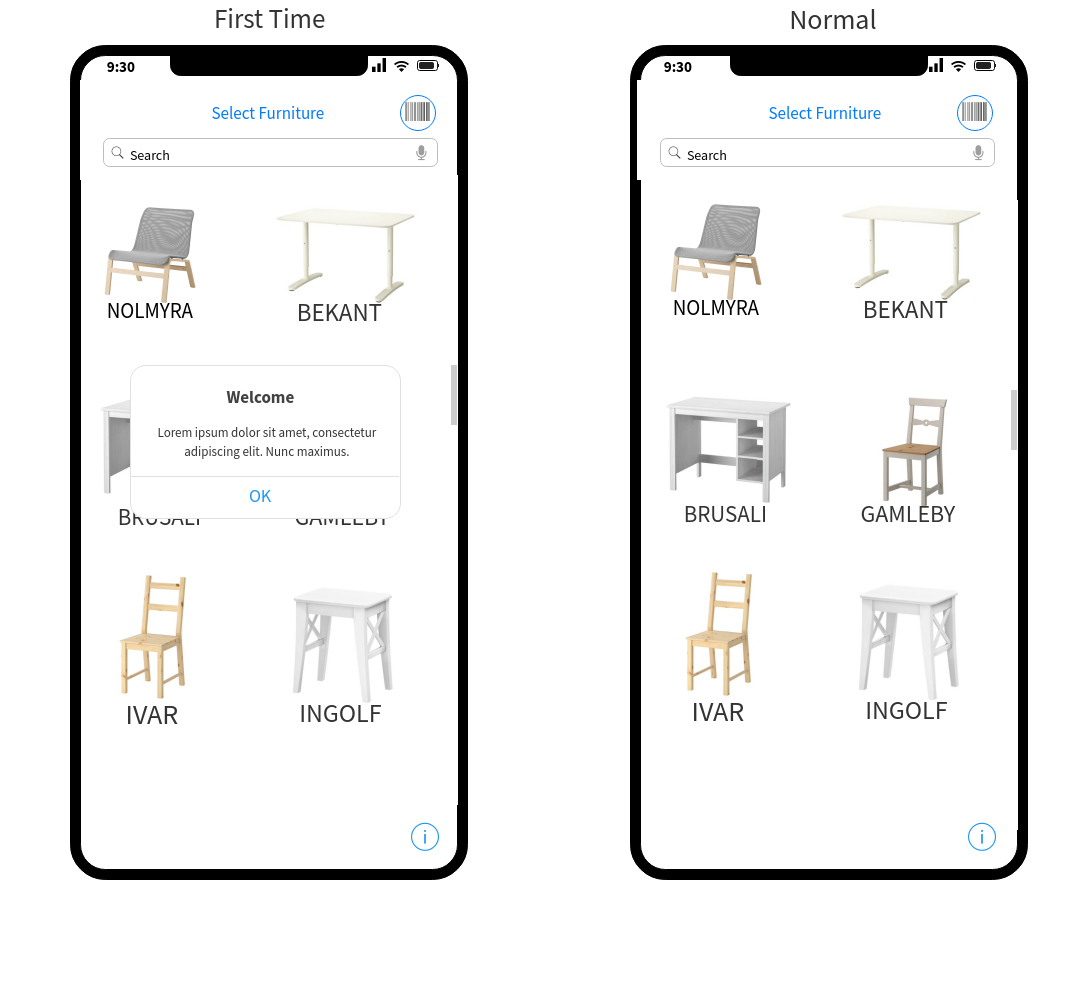
\includegraphics[height = 0.4\textheight]{./Images/Furniture_Select.png}
\caption{Furniture selection screen which the user is greeted with when starting the application. The left image shows how it looks for first time users, and right side how it looks for known users.}
\label{fig:furniture-select}
\end{center}
\end{figure}

After selecting a furniture the user is taken to a detail view, figure \ref{fig:detail-view}. This view is there for the user to see bigger images of the furniture and its unique article number. This is useful since some furniture models look very similar. Here the user can also read other specific information about the piece of furniture as well as preview a 3D model of the furniture, showing how it will look like when it's completed. Once the user is ready, they are supposed to press the "Assemble" button to progress.
 
\begin{figure}[hbtp]
\begin{center}
\includegraphics[height = 0.4\textheight]{./Images/Detail_view.png}
\caption{.}
\label{fig:detail-view}
\end{center}
\end{figure}


In the Assemble view the user is greeted with a live feed camera view as well as an information field containing instructions, see figure \ref{fig:assemble-view}. The first step for the user is to scan the pieces on the floor, allowing the machine learning model to find the pieces that are supposed to be assembled. Once the first parts are automatically found, they are highlighted using bounding boxes to alert the user of their current importance. The user can then press the "Next" button to continue. Afterwards, an animation showing the 3D parts in question being assembled properly and informatively. When the user has put together the parts, they press "Next". This process will then be fed with the next set of instructions and will continue like this until the	 piece of furniture is fully assembled.
\begin{figure}[hbtp]
\begin{center}
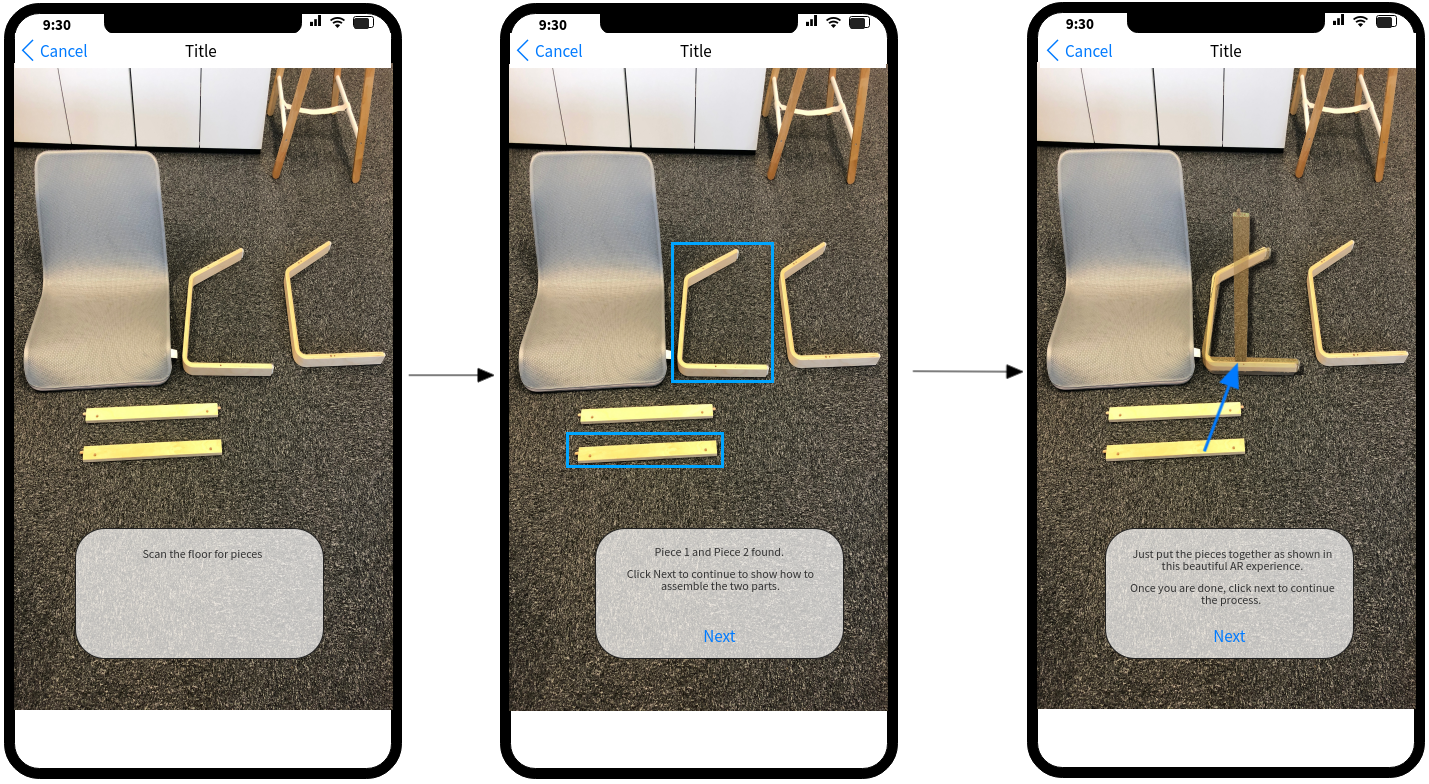
\includegraphics[height = 0.4\textheight]{./Images/AR_Scene.png}
\caption{Shows from left to right the user flow of putting two pieces together.}
\label{fig:assemble-view}
\end{center}
\end{figure}

\newpage